

%	Mia Gerber 
%	15016502
%	
%	COS 301: Assignment 2
%
%	Navigation Subsystem: Requirements, Constraints and Attributes


	
	\subsection{External Interface Requirements}
	 \textbf{ These requirements relate to both interfacing with other subsystems within the UP Nav system as well as interfacing with the hardware that the application will be deployed on.}
	 \begin{table}[H]
	 	\centering
	 	\caption{Navigational Information}
	 	\label{my-label}
	 	\resizebox{\textwidth}{!}{%
	 		\begin{tabular}{|l|l|}
	 			\hline
	 			Name                  & Navigational Information                                                                                                                                                                                                                                                                                                 \\ \hline
	 			Description           & \begin{tabular}[c]{@{}l@{}}This is the, navigational data that allows the user to navigate around campus. \\ More, specifically with regards to fitness this data will allow us to keep track \\ of, distances and allow fitness statistics to be drawn from the distances, \\ travelled during navigation.\end{tabular} \\ \hline
	 			Source \& Destination & Source:Server, Destination: Device/Application                                                                                                                                                                                                                                                                           \\ \hline
	 			Range, accuracy       & \begin{tabular}[c]{@{}l@{}}The range of this information would be roughly (0-100km) as an estimate of \\ the absolute maximum someone would walk in a single day on campus.\end{tabular}                                                                                                                                 \\ \hline
	 			Unit of measure       & The unit of,measure for this specific data would be in kilometers.                                                                                                                                                                                                                                                       \\ \hline
	 			Timing                & \begin{tabular}[c]{@{}l@{}}The information will be kept on device until such a point that the user logs out \\ or uninstalls. The Information will be kept on server until such a point that the \\ user deletes their account.\end{tabular}                                                                             \\ \hline
	 			Relations to other    & \begin{tabular}[c]{@{}l@{}}This information relates to ‘fitness information’ because the distances travelled \\ during navigation are to be used in calculating the number of steps made and is \\ crucial in the calculations of calories burned and other fitness statistics that are \\ calculated.\end{tabular}      \\ \hline
	 			Data format           & \begin{tabular}[c]{@{}l@{}}The format,of this would be stored in a float value as to allow accuracy of \\ distances,travelled and would be transferred over JSON as to integrate with our \\ chosen, technology of using Cordova.\end{tabular}                                                                           \\ \hline
	 		\end{tabular}%
	 	}
	 \end{table}
	\begin{itemize}
		\small
		\item To "Notifications" module will be used to give directions to the user during navigation in the form of push notifications.
		\item The "Points of interest" module will be seen by the Navigation module simply as destinations to be navigated to or as a current location.
		\item The GIS module will be used continually throughout navigation and as such is included in most of the UML diagrams, because of this tight coupling, implementation of the system needs to be done in a way that ensures easy communications between these two subsystems.
		\item Interfacing with the user's mobile device will be done with a cross platform API, explained in the "Technologies" section.
	\end{itemize}
	
	\subsection{Performance Requirements}
	\begin{itemize}
		\small
		\item Immediate response in the form of a notificaiton if user goes off route
		\item User can choose if application can continue navigation in the background even if the application isn't currently open. (Optional background data usage)
		\item "Fuzzy searching" when user is looking for a destination and misspells a word the application can still recognise the intended destination and navigate to the correct place.
		\item Navigation seamlessly continues when user suddenly changes from using campus wifi to using mobile data. (Interaction between GIS module and Navigation module is important here.)
	\end{itemize}
	
	\subsection{Design Constraints}
	\begin{itemize}
		\small
		\item The use of design patterns is crucial to object oriented software engineering but we are limited 
			in the types of design patterns we are able to use within the subsystems due to the requirements 
			imposed upon the system as a whole.
		\item The Navigation subsystem receives critical information from the GIS subsystem to ensure that the route
			calculated is correct and to recalculate the route in real time if the user goes off track. The coupling between these two modules will be high and might affect the implementation of other subsystems that also rely upon GIS information.
		\item Our application will be deployed across multiple platforms using different GIS implementations forcing the Navigation module to be able to perform uniformly when receiving coordinates in different formats or encodings.
		\item Users will want to limit the amount of data transfer occurring when using the application, the only way to implement this is to restrict communication with the server and database which could impact navigation efficiency and user experience.
	\end{itemize}
	
	\subsection{Software System Attributes}
	\begin{itemize}
		\small 
		\item High cohesion with low coupling allowing for easy addition, removal or replacement of modules.
		\item Polymorphism will be implemented as means of specifying object behaviour when the user imposes restrictions upon the base behaviour of the object.
		\item All source files will be written in an Object Oriented capable language.
		\item We will need to interface with the user's device at a level capable of accessing push notifications and 
		 GIS data.
	\end{itemize}
	
	\subsection{Class Diagram}
	\begin{figure}[H]
	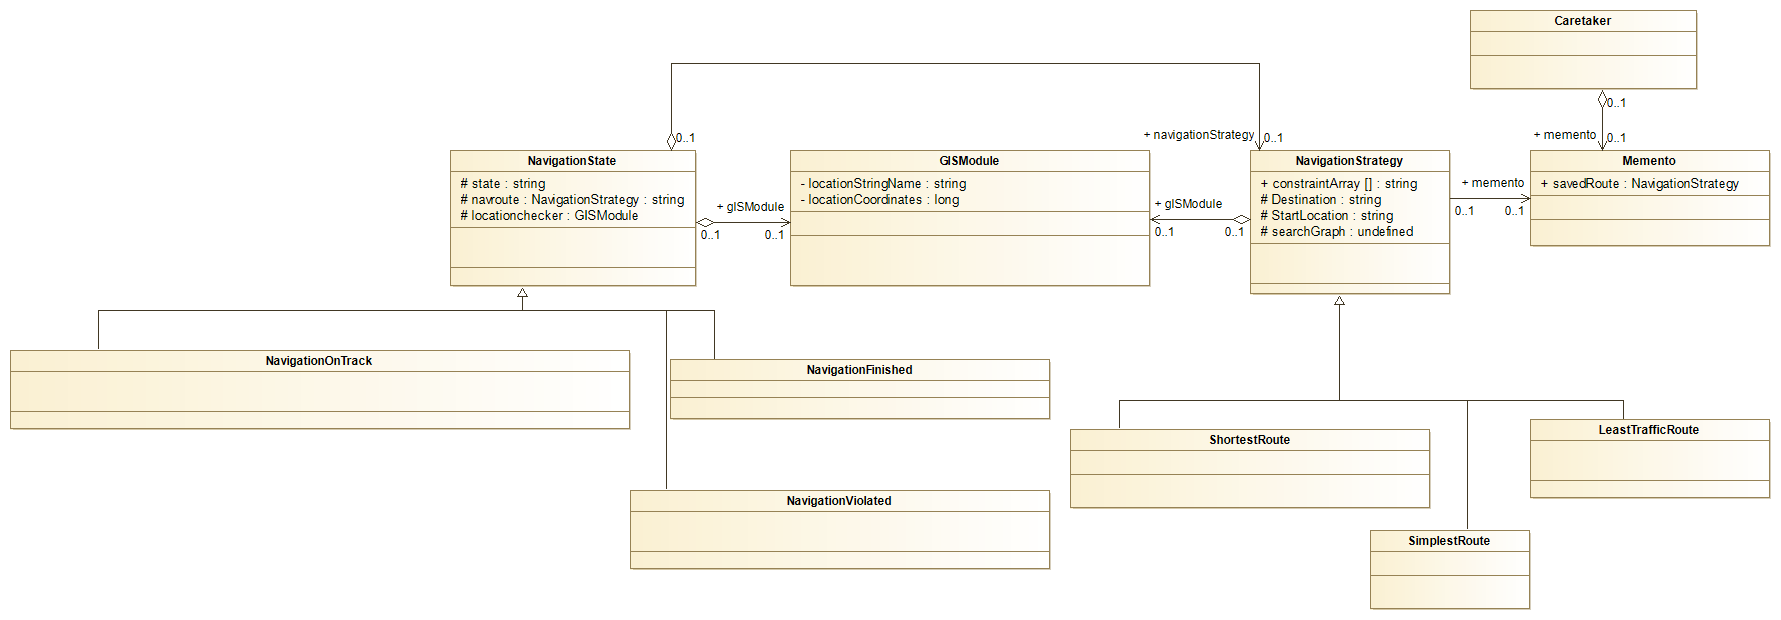
\includegraphics[width=\linewidth]{Navigation/NavigationModuleClassDiagram(v2_noMethods).png}
	\caption{Navigation Class Diagram}
	\label{fig:UML1}
	\end{figure}
	
	\subsection{Design Patterns used}
	\paragraph{Discussion of design patterns implemented in UML diagrams:}
		Memento: To save a route for future use
		
		Splitting the functions of the Navigation module essentially leaves us with two structures within the module. An internal state that is constantly changing as well as a means of navigations (different algorithms to achieve navigation to destination). Keeping this in mind I decided to use the State and Strategy design patterns, these design patterns both function on the same basic principal of modularity and separation of concerns. Additionally, because the Strategy design pattern represents what is essentially a list of directions, if the user decides to save their route so that they may return to it later, the Memento design pattern was included to ensure sensible safekeeping.
		
		There are three possible states, namely: "Navigation in progress", "Navigation has been violated" and "Navigation exited successfully". Each one of these states interacts with the chosen strategy in a different way. which is why there is aggregation between the State and Strategy classes.
		
		The Strategy class and its subclasses will deal with user constraints by keeping an array of said constraints and constructing a graph using information gathered from both the GIS Module as well as user input to ensure graph traversal will result in a desirable route. 
	
	\subsection{Activity Diagram}
	\begin{figure}[H]
	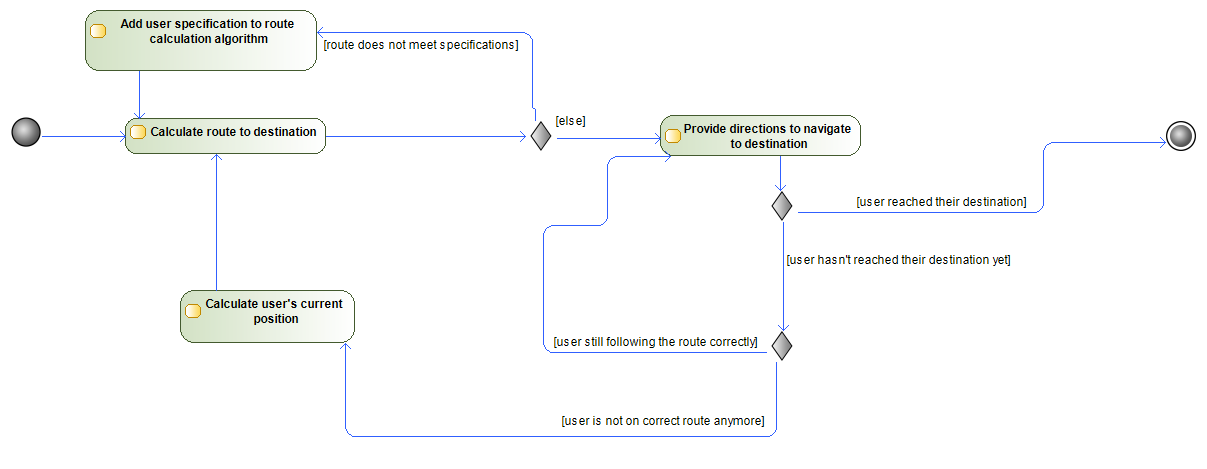
\includegraphics[width=\linewidth]{Navigation/NavigationModuleActivityDiagram.png}
	\caption{Navigation Activity Diagram}
	\label{fig:UML2}
	\end{figure}
	
	\subsection{Sequence Diagram}
	\begin{figure}[H]
	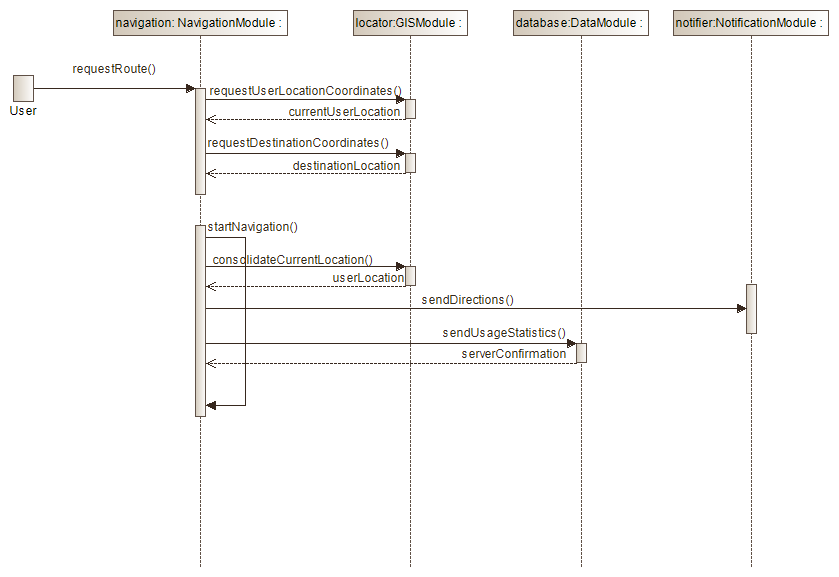
\includegraphics[scale=0.44]{Navigation/NavigationModuleSequenceDiagram.png}
	\caption{Navigation Sequence Diagram}
	\label{fig:UML5}
	\end{figure}
	
	\subsection{State Diagram}
	\begin{figure}[H]
	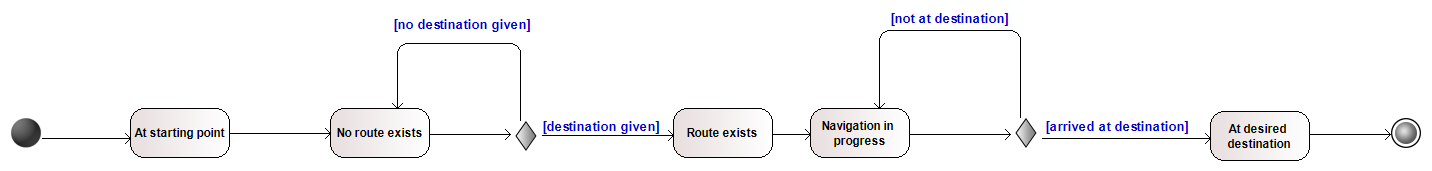
\includegraphics[width=\linewidth]{Navigation/NavigationModuleStateDiagram.png}
	\caption{Navigation State Diagram}
	\label{fig:UML3}
	\end{figure}
	
	\subsection{Use Case Diagram}
	\begin{figure}[H]
	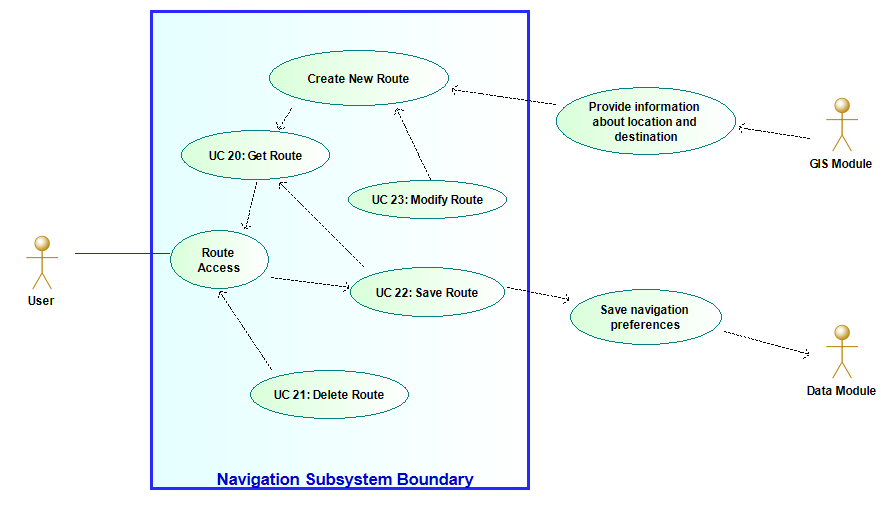
\includegraphics[width=\linewidth]{Navigation/NavigationModuleUseCaseDiagram.png}
	\caption{Navigation Use Case Diagram}
	\label{fig:UML4}
	\end{figure}
	
	


	
	
	

